\section{Extra figures and implementation details}
\label{appendix:A1}
This section contains additional details on the implementation, and supplementary figures of the fitted models. For details and figures belonging to Section \ref{section:Application1}, see Section \ref{appendix:application1}, and for Section \ref{section:application2} see Section \ref{appendix:application2}.

\subsection{Extras of Section \ref{section:Application1}}
\label{appendix:application1}
\subsubsection{Extra figures}
\label{appendix:figures}

\begin{figure}[h!]
    \centering
    \begin{subfigure}[b]{\textwidth}   
        \centering 
        \caption[]%
        {}    
        \label{figure:Application1:rw2_age_f}
        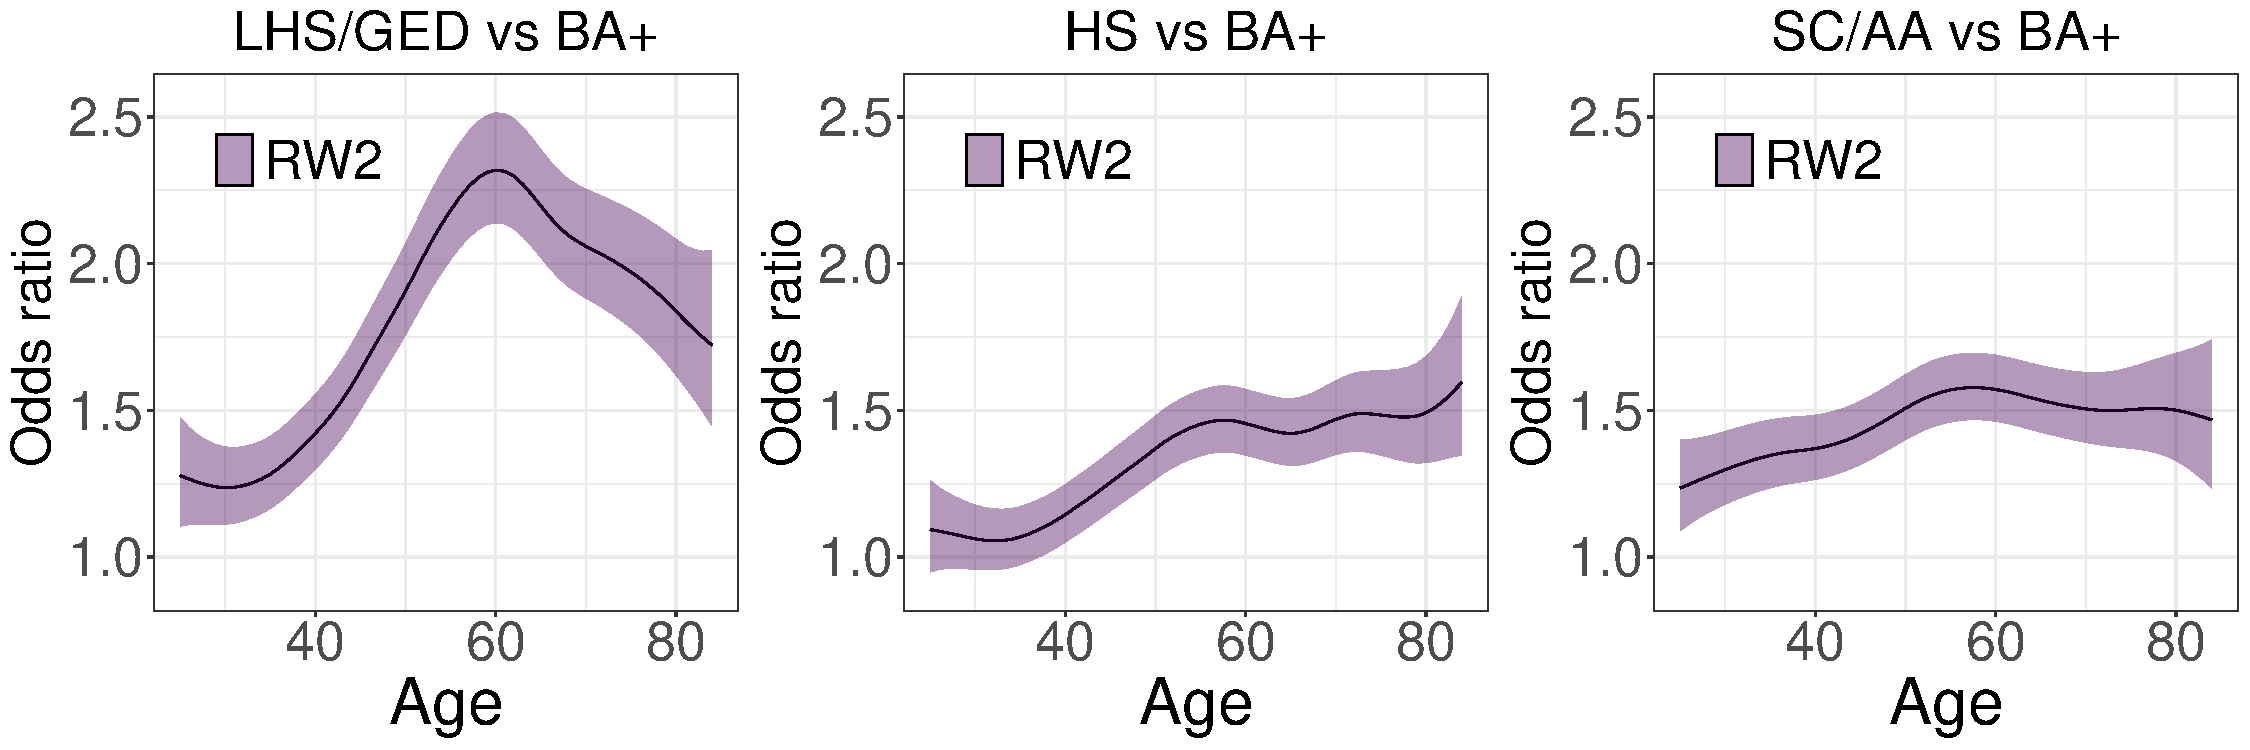
\includegraphics[width=\textwidth]{Figures/rw2_age_f.pdf}
    \end{subfigure}
    \vskip\baselineskip\vspace{-0.3cm}
    \begin{subfigure}[b]{\textwidth}   
        \centering 
        \caption[]%
        {}    
        \label{figure:Application1:rw2_cohort_f}
        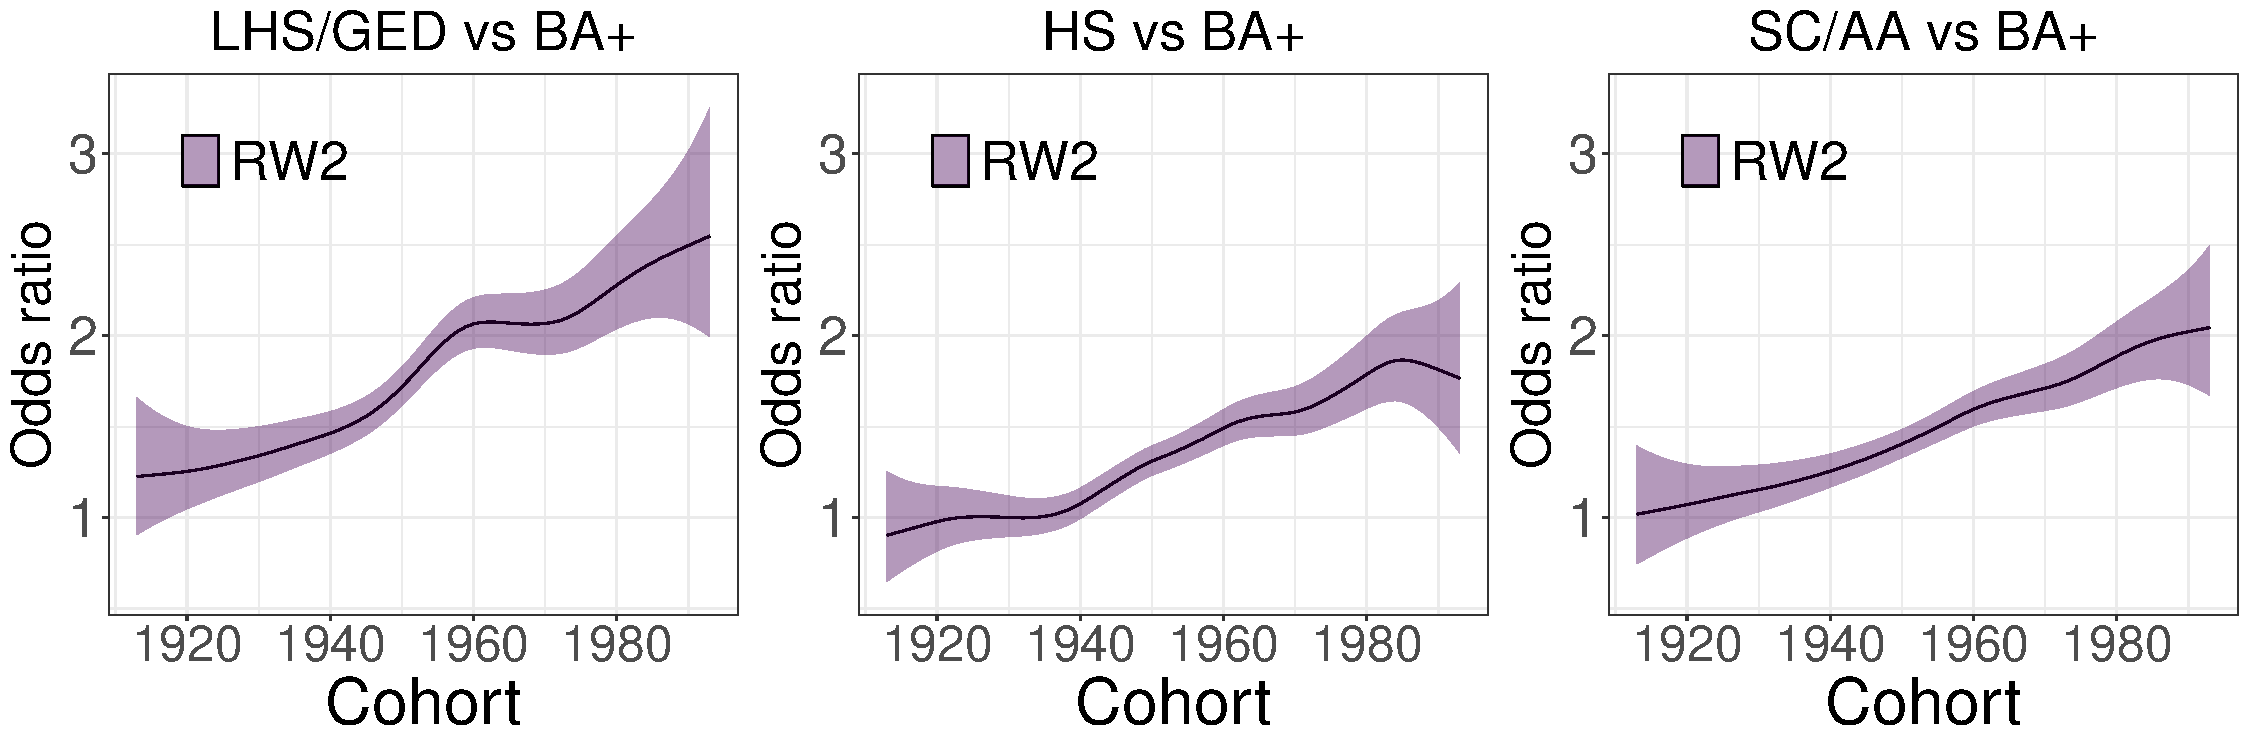
\includegraphics[width=\textwidth]{Figures/rw2_cohort_f.pdf}
    \end{subfigure}
    \caption{The posterior estimated median odds-ratio over (a) age and (b) cohort, for different levels of attained education with respect to the highest level of education, along with a $95\%$ credible interval for an aPc model, using female data and RW2 priors for each temporal component in the latent field. A PC$(10,0.01)$ prior is placed on the standard deviation of each component.}
    \label{figure:Application1:rw2_f}
\end{figure}

\captionsetup[subfigure]{labelfont={bf,large}, font={large}, skip=1pt, margin=0cm, singlelinecheck=true}

%Compare standard deviation plot for male data
\begin{figure}[h!]
    \centering
    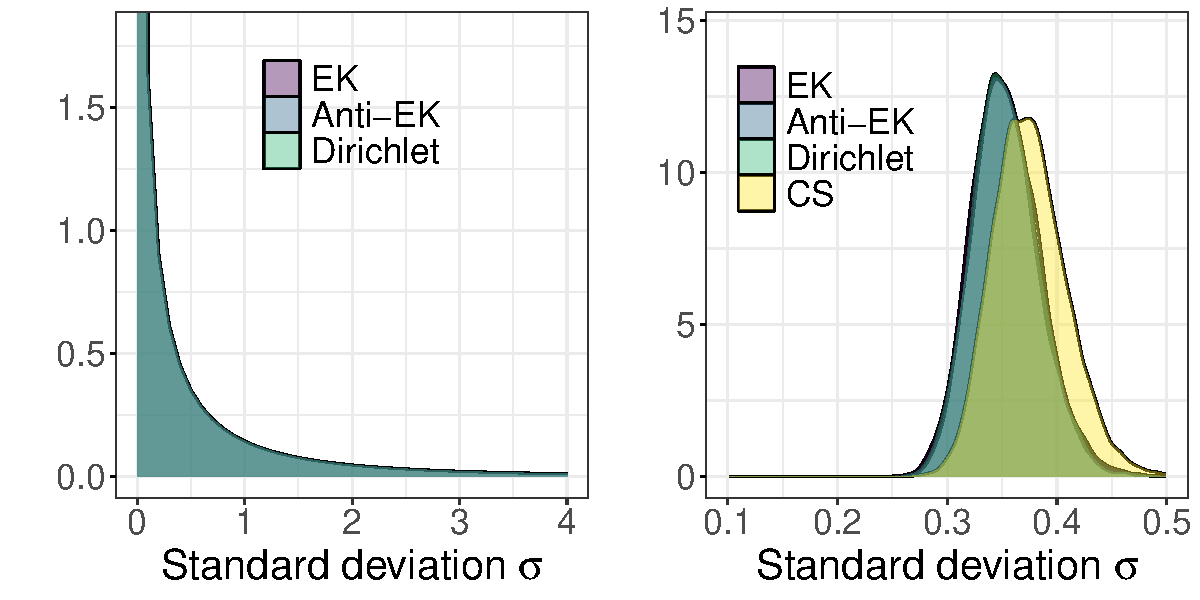
\includegraphics[width=0.8\textwidth]{Figures/compare_plots_s0_m.pdf}
    \caption{The prior (left) and posterior (right) distributions of the standard deviation in aPc models using male data along with expert knowledge (EK), anti-EK, Dirichlet, and component-specific (CS) priors outlined in Section \ref{section:application1:prior}. }
    \label{figure:Application1:s0_m}
\end{figure}

%Compare posterior plots for male data
\begin{figure}[h]
    \centering
    \begin{subfigure}[b]{0.8\textwidth}
        \centering
        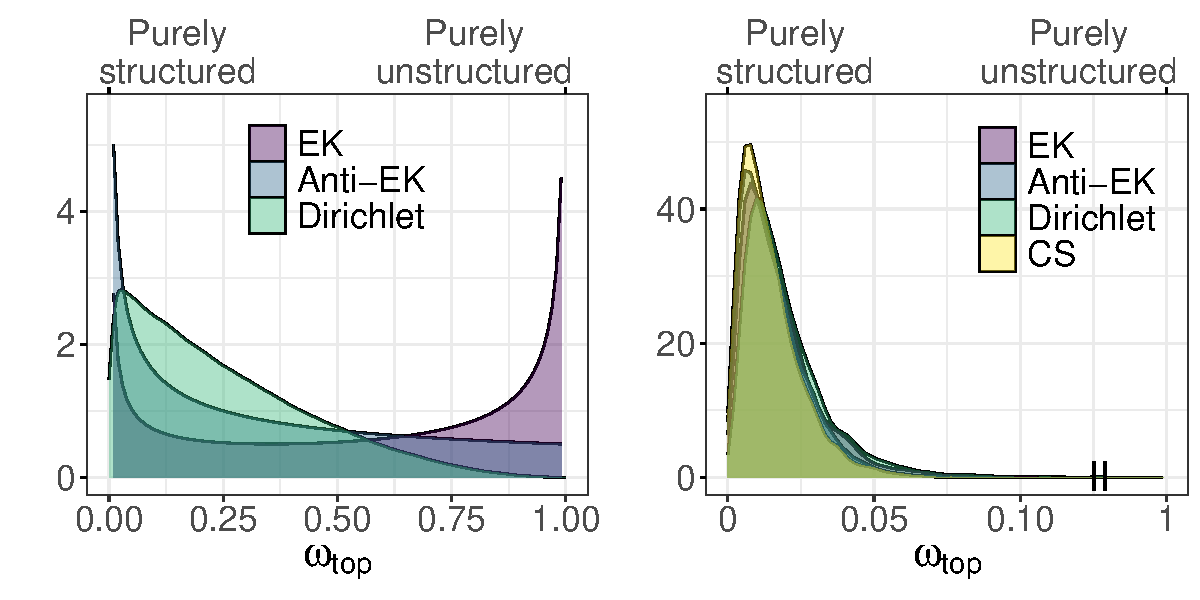
\includegraphics[width=\textwidth]{Figures/compare_plots_s1_m.pdf}
        \caption[Network2]%
        {{\small Top split}}    
        \label{figure:Application1:s1_m}
    \end{subfigure}
    \vskip\baselineskip\vspace{-0.5cm}
    \begin{subfigure}[b]{0.8\textwidth}   
        \centering 
        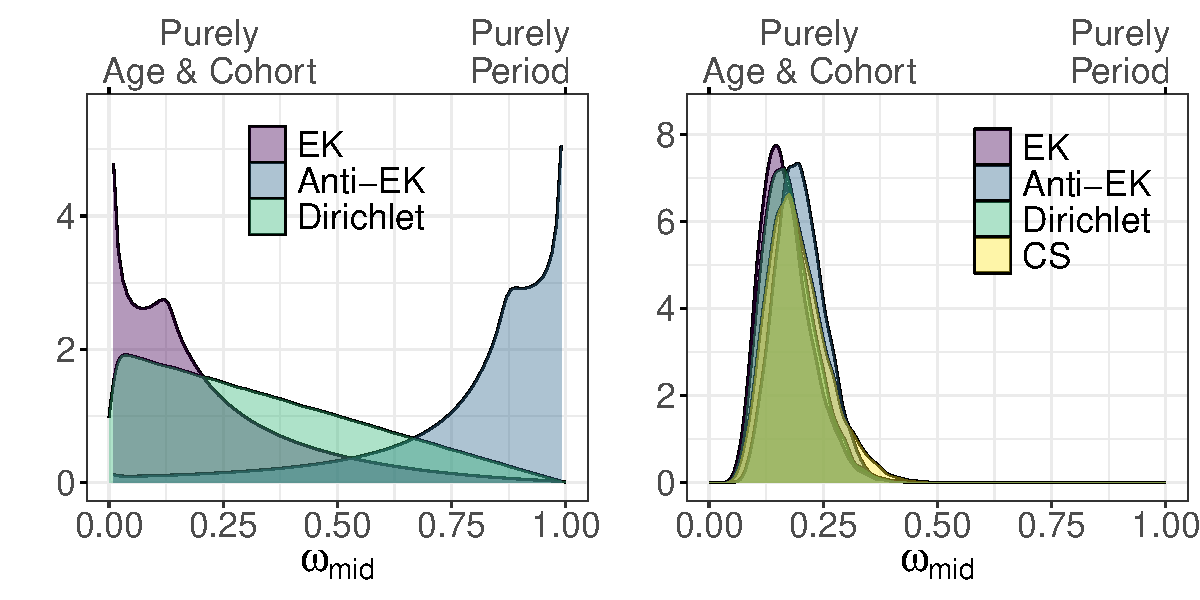
\includegraphics[width=\textwidth]{Figures/compare_plots_s2_m.pdf}
        \caption[]%
        {{\small Middle split}}    
        \label{figure:Application1:s2_m}
    \end{subfigure}
    \vskip\baselineskip\vspace{-0.5cm}
    \begin{subfigure}[b]{0.8\textwidth}   
        \centering 
        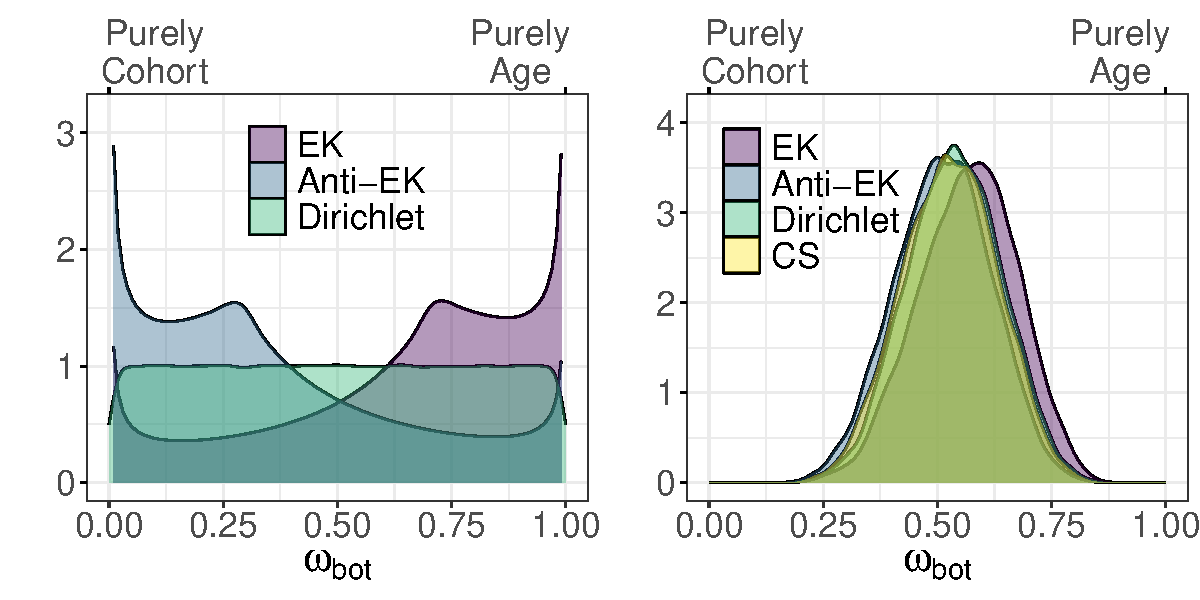
\includegraphics[width=\textwidth]{Figures/compare_plots_s3_m.pdf}
        \caption[]%
        {{\small  Bottom split}}    
        \label{figure:Application1:s3_m}
    \end{subfigure}
    \vspace{-0.2cm}
    \caption{The prior (left) and posterior (right) distribution of the mixing parameters at different levels in the hierarchical structure of the EK prior in aPc models using male data, and the expert knowledge (EK), anti-EK, Dirichlet, and component-specific (CS) priors outlined in Section \ref{section:application1:prior}. }
    \label{figure:Application1:compare-plots_m}

\end{figure}

\FloatBarrier
\subsubsection{Details on implementation in \texttt{R}}
\label{appendix:implementation:prior}
The \texttt{R} package \texttt{makemyprior} allows us to implement the desired hierarchical decomposition priors with the desired shrinkage, as outlined in Section \ref{section:application1:priorspecification}, although some additional modifications to the integration between \texttt{makemyprior} and \texttt{INLA} had to be made in order to implement the desired structure of the EK prior. Below follows an explanation of the procedure.

%What measures was taken differently
As mentioned in Section \ref{section:application1:priorspecification}, due to the stratification by education, the stratum specific effects inherently require an additional weight parameter to split the variance between each stratum. This property is undesirable as it requires incorporation of prior beliefs on how the different strata explain the variance. The provided EK does not provide intuition on how this split should be made, and it is therefore desirable to perform computations on the levels in which EK is provided. As such, the resolution done here is to have the computational software compute at this level by providing priors and evaluation functions that facilitate this. To achieve this, the prior made in \texttt{makemyprior} has to recognize only one node for each stratum specific effect, and for the computed precision (inverse variance) of the four stratified random effects to be evaluated jointly in \texttt{INLA}. 

In \texttt{makemyprior}, random effects are specified in R-formula syntax using the \texttt{mc()} function which has similar functionality to the function \texttt{f()} found in \texttt{INLA}. For each of the age, period and cohort effects, the desired latent RW1 prior structure is specified using the option \texttt{model = "rw1"}. This way, stratum specific effects require four RW1 specifications, though for the sake of the prior we wish to have a single specification. To circumvent this, a user specified precision structure matrix is created using the Kronecker product with the $4\times 4$ identity matrix and the RW1 structure matrix shown in Equation \eqref{eqn:rw1-structure-matrix}. This matrix then contains the structure matrix for four independent RW1 effects, one for each of the four strata, modelled as one matrix. This matrix may then be used in a joint prior specification with a single precision as desired. The next step is to transform the indices from the four set of indices to run over the newly constructed matrix. As all of these sets of indices are of the same length, we consequently rearrange the indices to be $i'=i + e\cdot I$, where $e=1,2,3,4$ denotes the education level. Doing this for all the stratum specific effects, the random effect is modelled with the option \texttt{model = "generic0"} while supplying the new structure matrix as the \texttt{Cmatrix}. As a consequence, the stratum specific effect is evaluated as one effect in the prior. 

Next, \texttt{INLA} has to evaluate the four random effects generated by the stratification of a random effect as a single random effect, as the prior constructed with \texttt{makemyprior} suggests. To do this, the formula supplied to \texttt{INLA} will not use the matrix constructed above, but is provided a random effect for each stratum of a stratum specific effect. Using expert settings in \texttt{INLA}, we may supply \texttt{INLA} variations of the functions normally passed on by \texttt{makemyprior} to make sense of the joint prior specifications generated by \texttt{makemyprior}. To achieve the desired result, the precision evaluation function is modified to pool the precision of the random effects before computations, meaning the computations are preformed on the parent node level, and not at the leaf node level. In \texttt{INLA}, the precisions of the random effects are given as log-precisions, meaning that the pooling is achieved by transforming to precisions, summing them, and then transforming back to log-precisions. 

\FloatBarrier
\subsubsection{Linear combinations in \texttt{INLA}}
\label{appendix:implementation:lincombs}
A full example of how the linear combinations are specified in \texttt{R} using \texttt{INLA} with toy-data is included in the Github repository of the thesis (\url{https://github.com/Markutr/MasterThesis}). Here, we give some a high-level overview of how it is done.

In \texttt{INLA}, a linear combination of random and fixed effects are specified using the function \texttt{inla.make.lincomb()}. Let us consider a simple case with three age groups, three periods and two education levels. We let $i$ $(i= 1,2,3)$ denote the age groups, $j$ $(j= 1,2,3)$ denote the periods, $k$ $(k= 1,2,3,4,5)$ denote the cohorts, and $e$ $(e= 1,2)$ denote the level of education. Moreover, we consider an aPC model, where the age effect is education-specific and the period and cohort effects are shared between stratum. We let $\mu_e$ denote the education-specific intercept, $\theta_{ie}$ denote the age effect, $\phi_j$ denote the period effect, $\psi_k$ denote the cohort effect and $\varepsilon_{ije}$ denote an unstructured effect. Finally, we model the probabilities $\pi_{ije}$ on a logit scale. The linear predictor (akin to Equation \eqref{eqn:linear-pred}) defining the model is then
\begin{equation}
    \text{logit}(\pi_{ije}) = \mu_e + \theta_{ie} + \phi_j + \psi_k + \varepsilon_{ije}.
\end{equation}
In our example here, we will be basing our explanation using the model specified in the \texttt{R} formula syntax:
\begin{lstlisting}
    formula = -1 + Education1 + Education2 + 
              f(Age_Education1, model = "rw1") + 
              f(Age_Education2, model = "rw1") +
              f(Period, model = "rw1") +
              f(Cohort, model = "rw1") +
              f(eps, model = "iid")
\end{lstlisting}
That is, the education-specific age effect is modelled as two separate random effects. 

\subsubsubsection*{Fixed effects}
In code, if the education-specific intercepts for the two education levels are given as "Education1" and "Education2" in the formula syntax, then we may specify a linear combination of their difference as
\begin{lstlisting}
    inla.make.lincomb(Education1 = 1, 
                      Education2 = -1)
\end{lstlisting}
Note that this corresponds to $\mu_1 - \mu_2$. If we wanted different coefficients (say $2\mu_1 - 0.1\mu_2$), then change the respective number in the function call. 

\subsubsubsection*{Random effects}
When passing data to \texttt{INLA}, each random effect is described over a set of indices. In our example, theses are provided in the given formula as "Age\_Education1", "Age\_Education2", "Period", "Cohort" and "eps". For each effect we wish to include in a linear combination, the \texttt{inla.make.lincomb()} function takes an array the length of this set of indices. The array is provided as a named argument with the same name as the set of indices it corresponds to. In this array, the random effect at the given position corresponds to random effect described at that position in the given indices. To omit effects, provide NA at the corresponding array positions. To include effects, provide the coefficient of the effect in the desired linear combination. For instance, say we wish to specify the linear combination describing the difference in the age effects between the strata for age group 2. Then, the formula is
\begin{lstlisting}
    inla.make.lincomb(Age_Education1 = c(NA,1,NA), 
                      Age_Education2 = c(NA, -1, NA))
\end{lstlisting}

\subsubsubsection*{Both fixed and random effects}
Linear combinations may be specified using both fixed and random effects at the same time (as done in our application). To do this, simply include the fixed and random effects as before. That is, 
\begin{lstlisting}
    inla.make.lincomb(Age_Education1 = c(NA,1,NA),
                      Age_Education2 = c(NA,-1,NA),
                      Education1 = 1,
                      Education2 = -1)
\end{lstlisting}


\subsubsection{Individual specific MAPC model}
\label{appendix:individual}
As argued in Section \ref{section:Application1}, the granularity of which we consider our analysis should not matter for anything other than computational time, as it is aggregated in \texttt{INLA}. To show this, a model was also fitted on the individual level data using the EK-prior derived in Section \ref{section:application1:prior}. Figure \ref{figure:Application2:lincombs_f_ind} shows the posterior median odds-ratio over age and cohorts in the aPc model using individual level data. The model using aggregated data (as in \ref{section:application1:results}) is also included to show that they are identical. Moreover, Figure \ref{figure:INDI:s0_f} shows the posterior distribution of the total variance $\sigma^2$ along with the prior, showing nearly identical posteriors for both models. Figure \ref{figure:INDI:compare-plots_f} shows the posterior distributions of the mixing parameters $\omega_{\text{top}}$, $\omega_{\text{mid}}$ and $\omega_{\text{bot}}$ (as described in \ref{section:application1:priorspecification}) based on $10,000$ samples, at each split of the prior tree structure used to formulate the EK-Prior. From these figures it is clear that the models provide the same fit, and for practical purposes are the same. Individual-specific covariates are therefore straightforward to include in future research.

\captionsetup[subfigure]{labelfont={bf,large}, font={large}, skip=1pt, margin=0cm, singlelinecheck=false}
\begin{figure}[h!]
    \centering
    \begin{subfigure}[b]{\textwidth}   
        \centering 
        \caption[]%
        {}    
        \label{figure:Application2:age_diff_f_ind}
        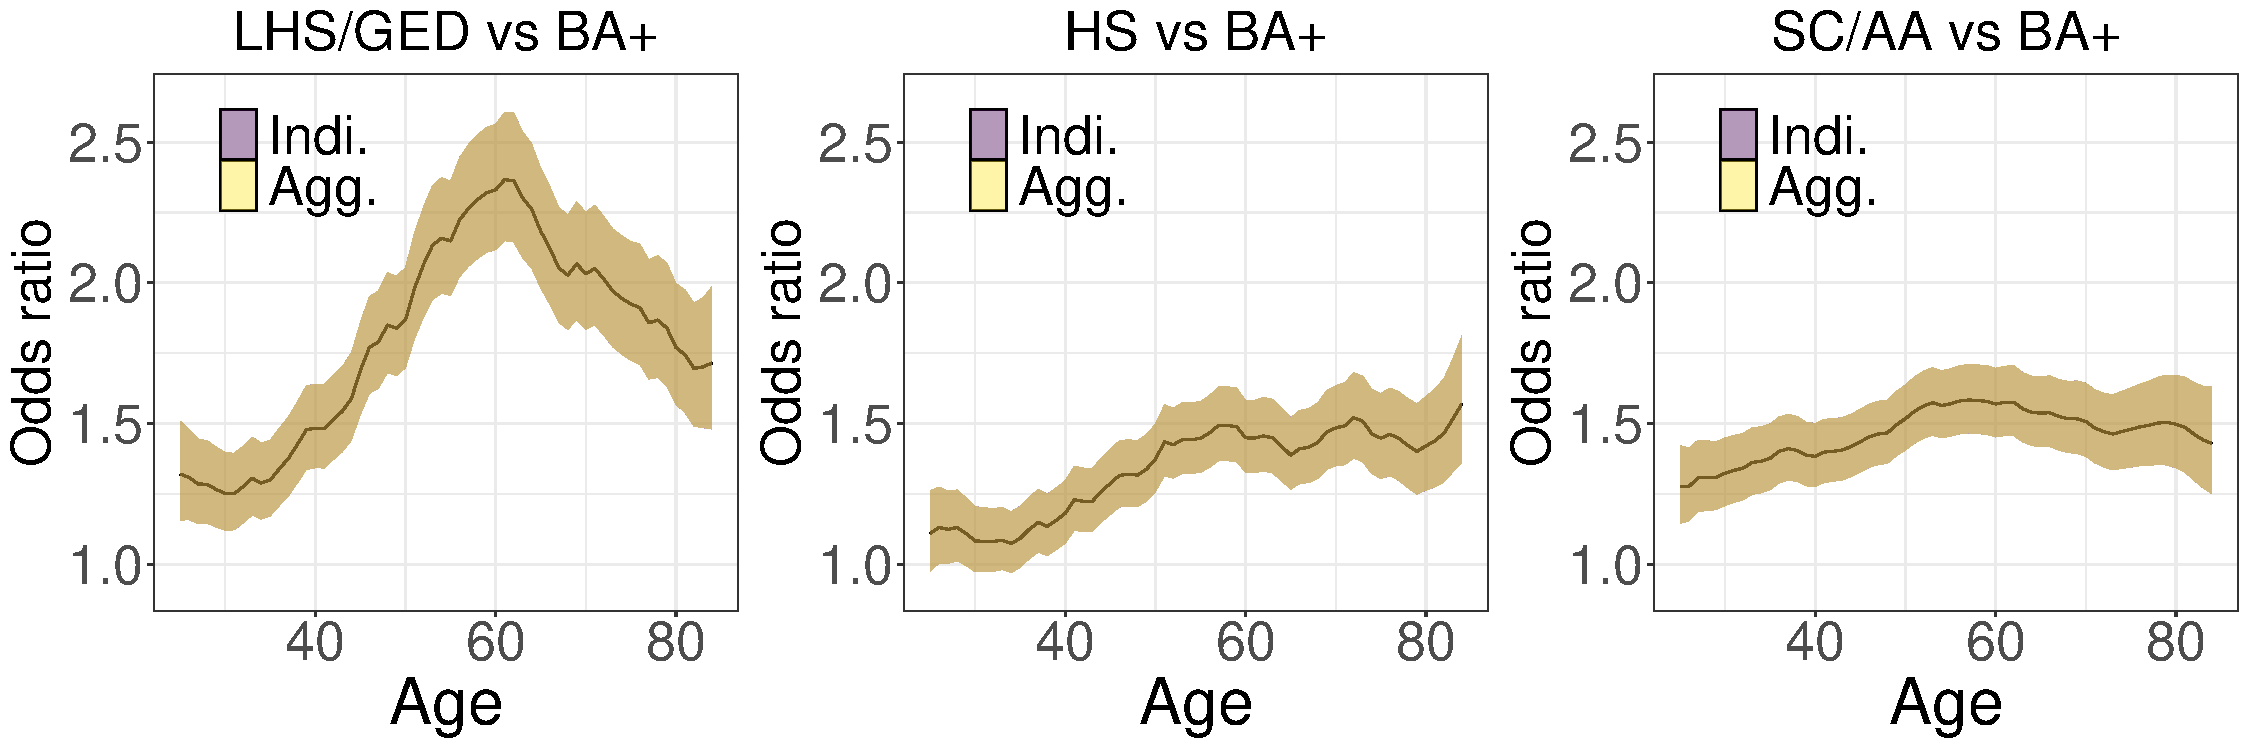
\includegraphics[width=\textwidth]{Figures/lincomb_ind_agg_m_age.pdf}
    \end{subfigure}
    \vskip\baselineskip\vspace{-0.3cm}
    \begin{subfigure}[b]{\textwidth}   
        \centering 
        \caption[]%
        {}    
        \label{figure:Application2:cohort_diff_f_ind}
        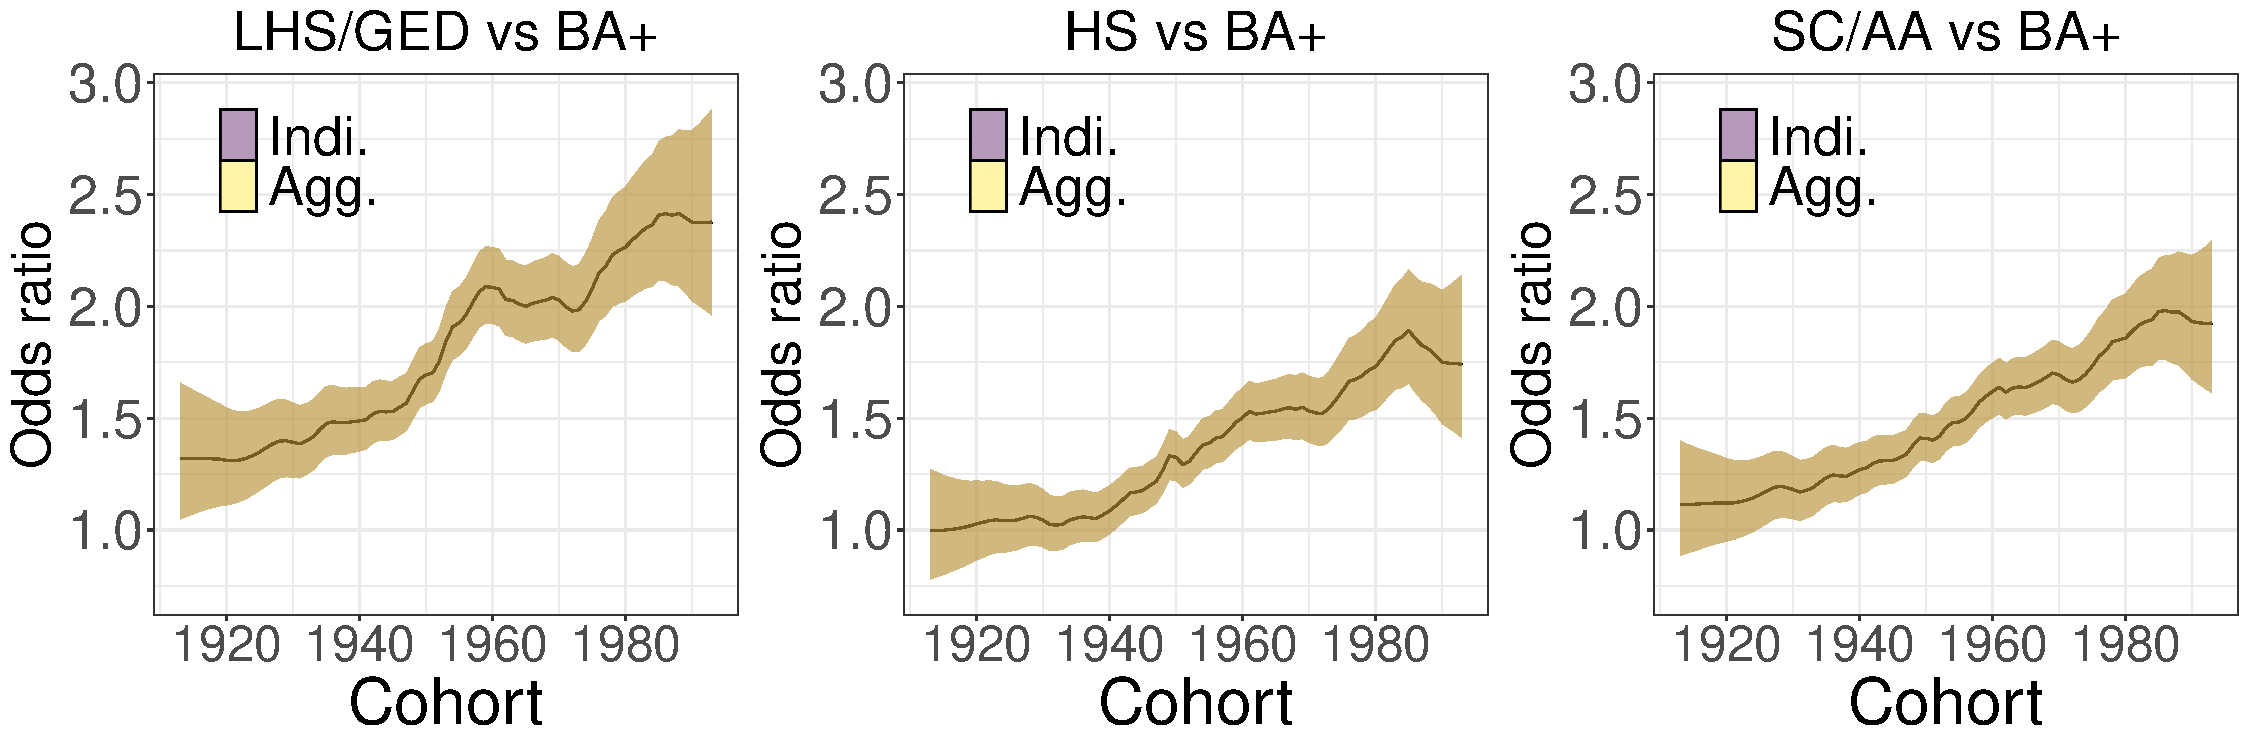
\includegraphics[width=\textwidth]{Figures/lincomb_ind_agg_m_cohort.pdf}
    \end{subfigure}
    \vspace{-0.2cm}
    \caption{The estimated difference in (a) age effects and (b) cohort effects between education levels along with a $95\%$ credible interval, all with respect to education attained at level bachelor or higher for the models using the data in an individual-specific and aggregated form.}
    \label{figure:Application2:lincombs_f_ind}
\end{figure}

\captionsetup[subfigure]{labelfont={bf,large}, font={large}, skip=1pt, margin=0cm, singlelinecheck=true}
%INDIVIDIAL S0
\begin{figure}[h!]
    \centering
    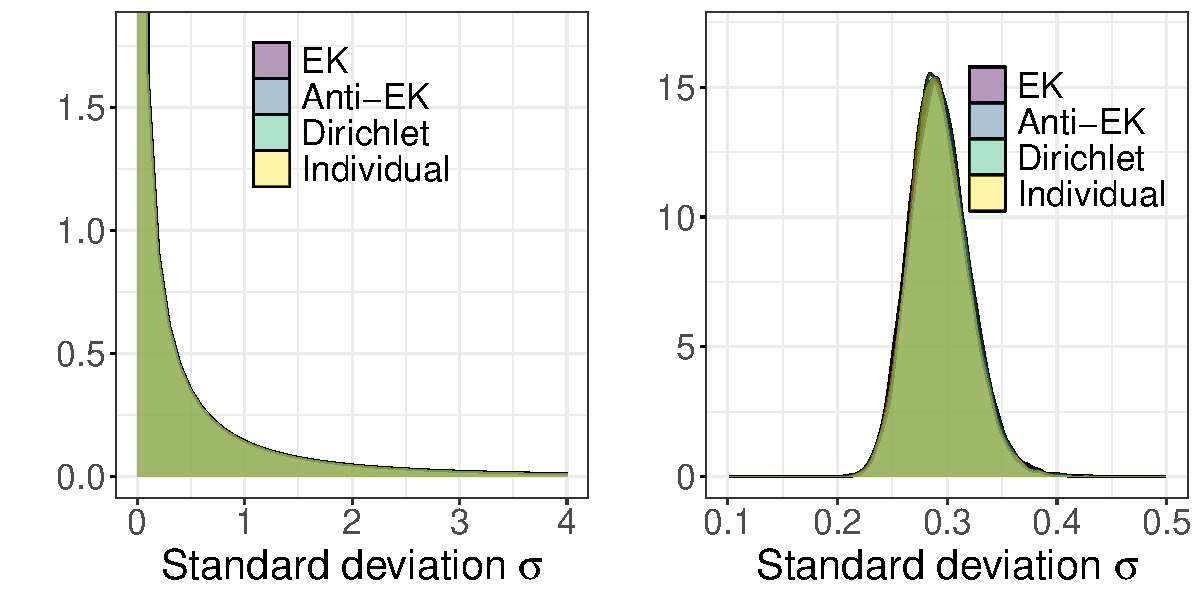
\includegraphics[width=0.8\textwidth]{Figures/compare_plots_indi_s0_f.pdf}
    \caption{The prior (left) and posterior (right) distributions of the standard deviation in aPc models using female data along with the expert knowledge (EK), anti-EK, and Dirichlet priors outlined in Section \ref{section:application1:prior}. The posterior when using the data on an individual-specific format is also included, labelled as "Individual", and uses the EK prior.}
    \label{figure:INDI:s0_f}
\end{figure}

%INDIVIDUAL SPLITS
\begin{figure}[h]
    \centering
    \begin{subfigure}[b]{0.8\textwidth}
        \centering
        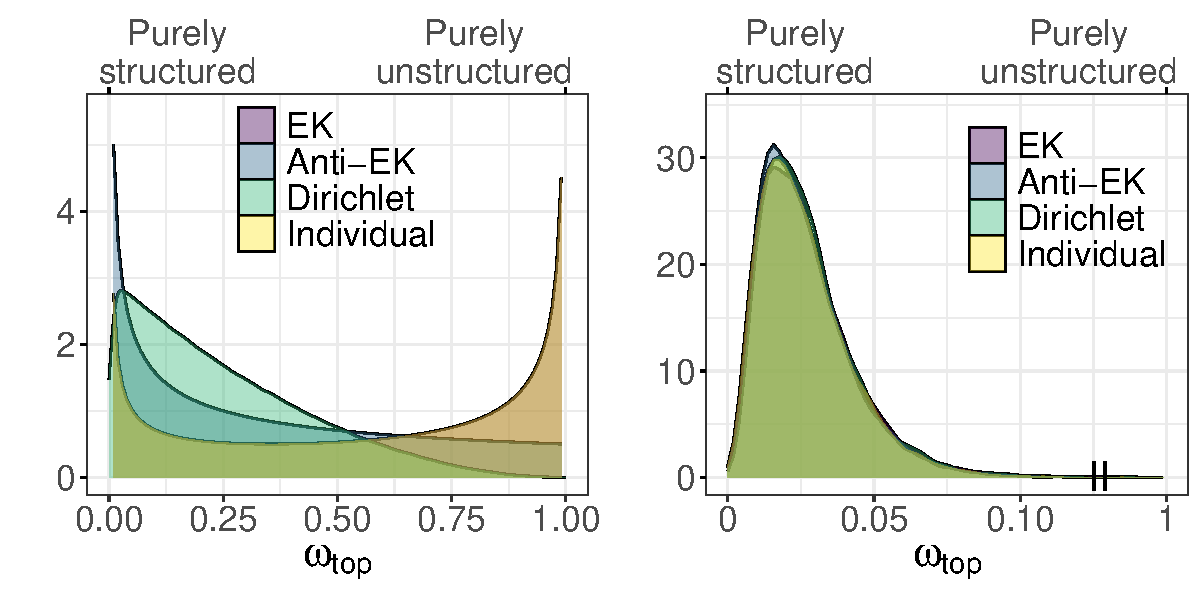
\includegraphics[width=\textwidth]{Figures/compare_plots_indi_s1_f.pdf}
        \caption[Network2]%
        {{\small Top split}}    
        \label{figure:INDI:s1_f}
    \end{subfigure}
    \vskip\baselineskip\vspace{-0.5cm}
    \begin{subfigure}[b]{0.8\textwidth}   
        \centering 
        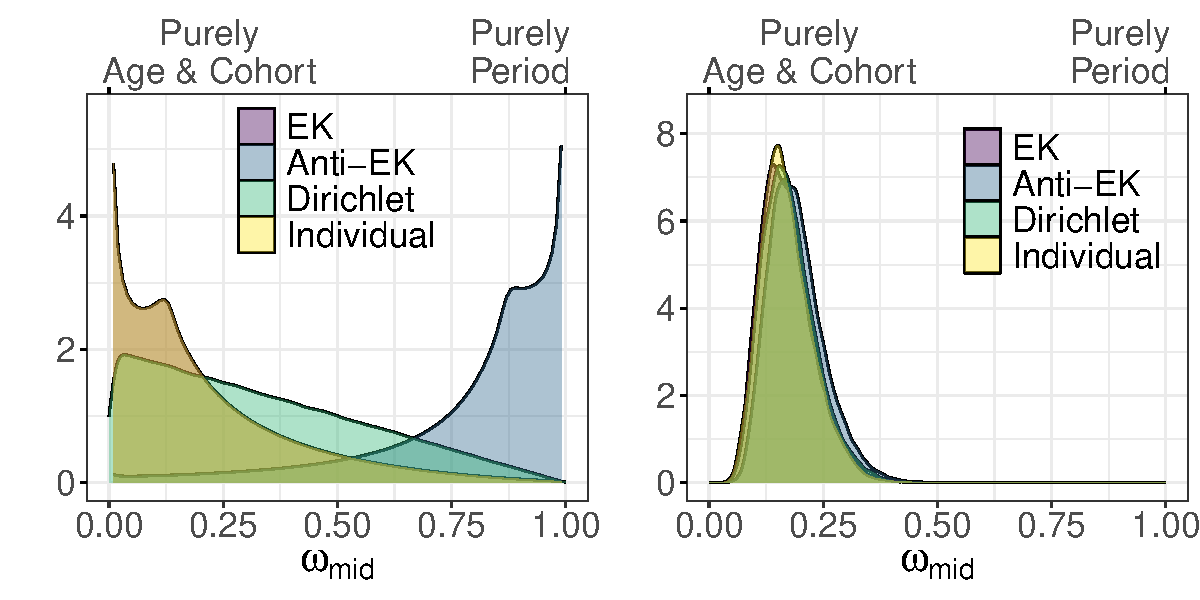
\includegraphics[width=\textwidth]{Figures/compare_plots_indi_s2_f.pdf}
        \caption[]%
        {{\small Middle split}}    
        \label{figure:INDI:s2_f}
    \end{subfigure}
    \vskip\baselineskip\vspace{-0.5cm}
    \begin{subfigure}[b]{0.8\textwidth}   
        \centering 
        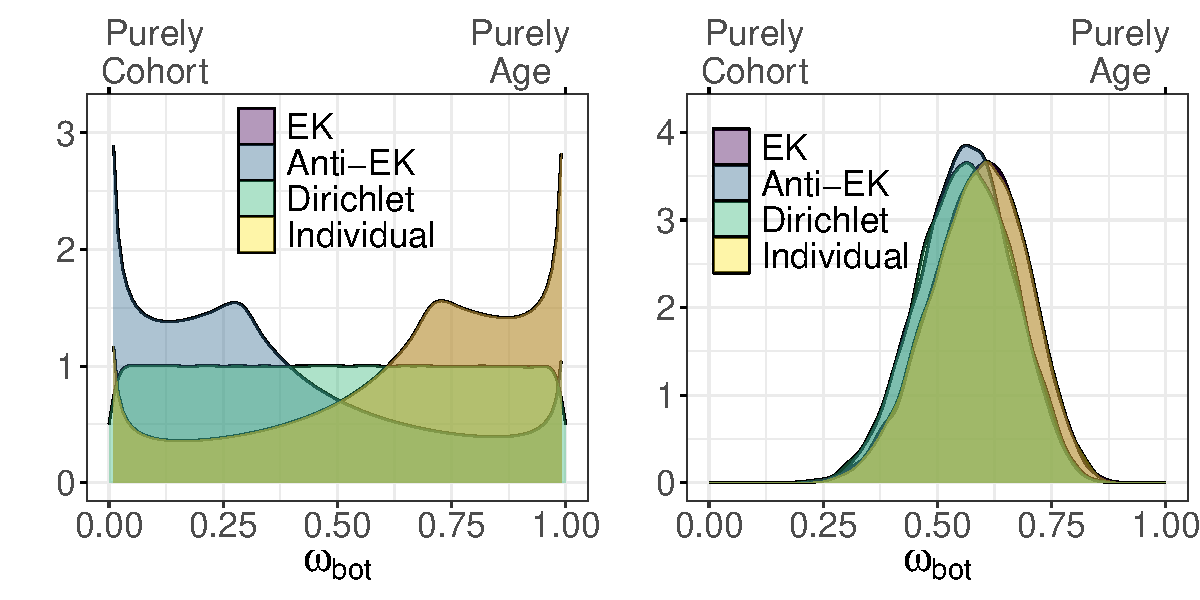
\includegraphics[width=\textwidth]{Figures/compare_plots_indi_s3_f.pdf}
        \caption[]%
        {{\small  Bottom split}}    
        \label{figure:INDI:s3_f}
    \end{subfigure}
    \vspace{-0.2cm}
    \caption{The prior (left) and posterior (right) distribution of the mixing parameters at different levels in the hierarchical structure of the EK prior in aPc models using female data and the expert knowledge (EK), anti-EK, and Dirichlet priors outlined in Section \ref{section:application1:prior}. The posteriors when using the data on an individual-specific format are also included, labelled as "Individual", and uses the EK prior.}
    \label{figure:INDI:compare-plots_f}
\end{figure}

\FloatBarrier
\subsection{Extras of Section \ref{section:application2}}
\label{appendix:application2}
\subsubsection{Extra figures}


\captionsetup[subfigure]{labelfont={bf,large}, font={large}, skip=1pt, margin=0cm, singlelinecheck=false}
\begin{figure}[h!]
    \centering
    \begin{subfigure}[b]{\textwidth}   
        \centering 
        \caption[]%
        {}    
        \label{figure:Application1:rw2_age_f_fil}
        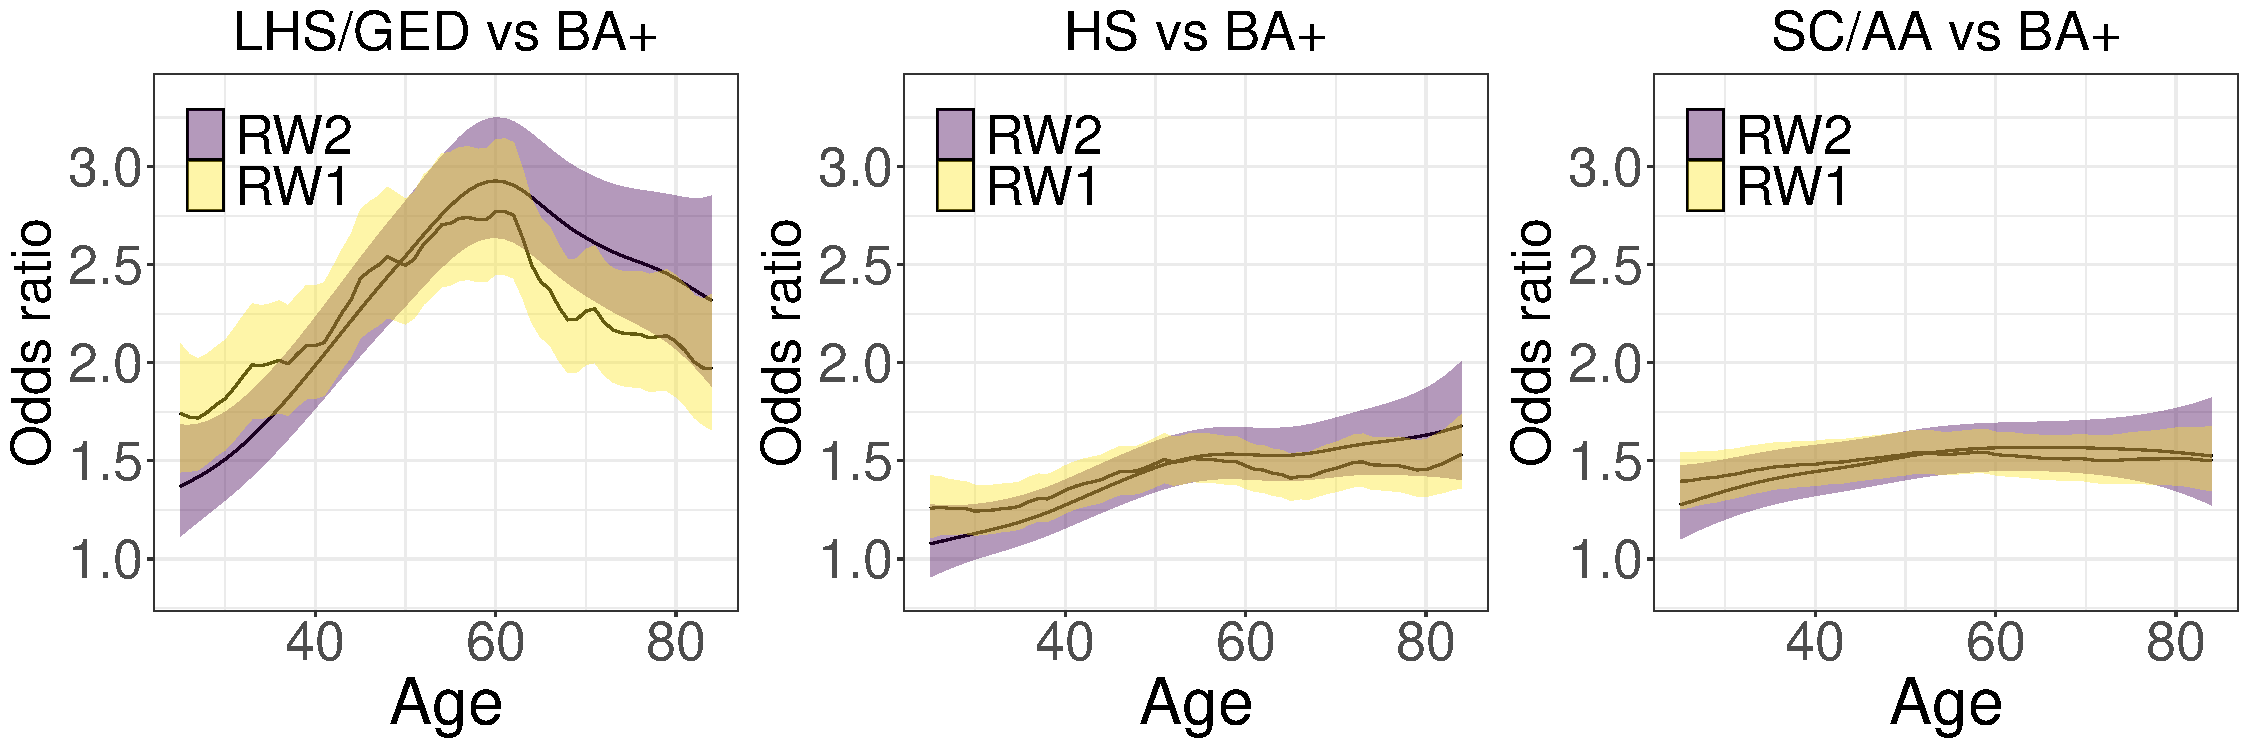
\includegraphics[width=\textwidth]{Figures/lincomb_survey_filtered_age_f_rw2.pdf}
    \end{subfigure}
    \vskip\baselineskip\vspace{-0.3cm}
    \begin{subfigure}[b]{\textwidth}   
        \centering 
        \caption[]%
        {}    
        \label{figure:Application1:rw2_cohort_f_fil}
        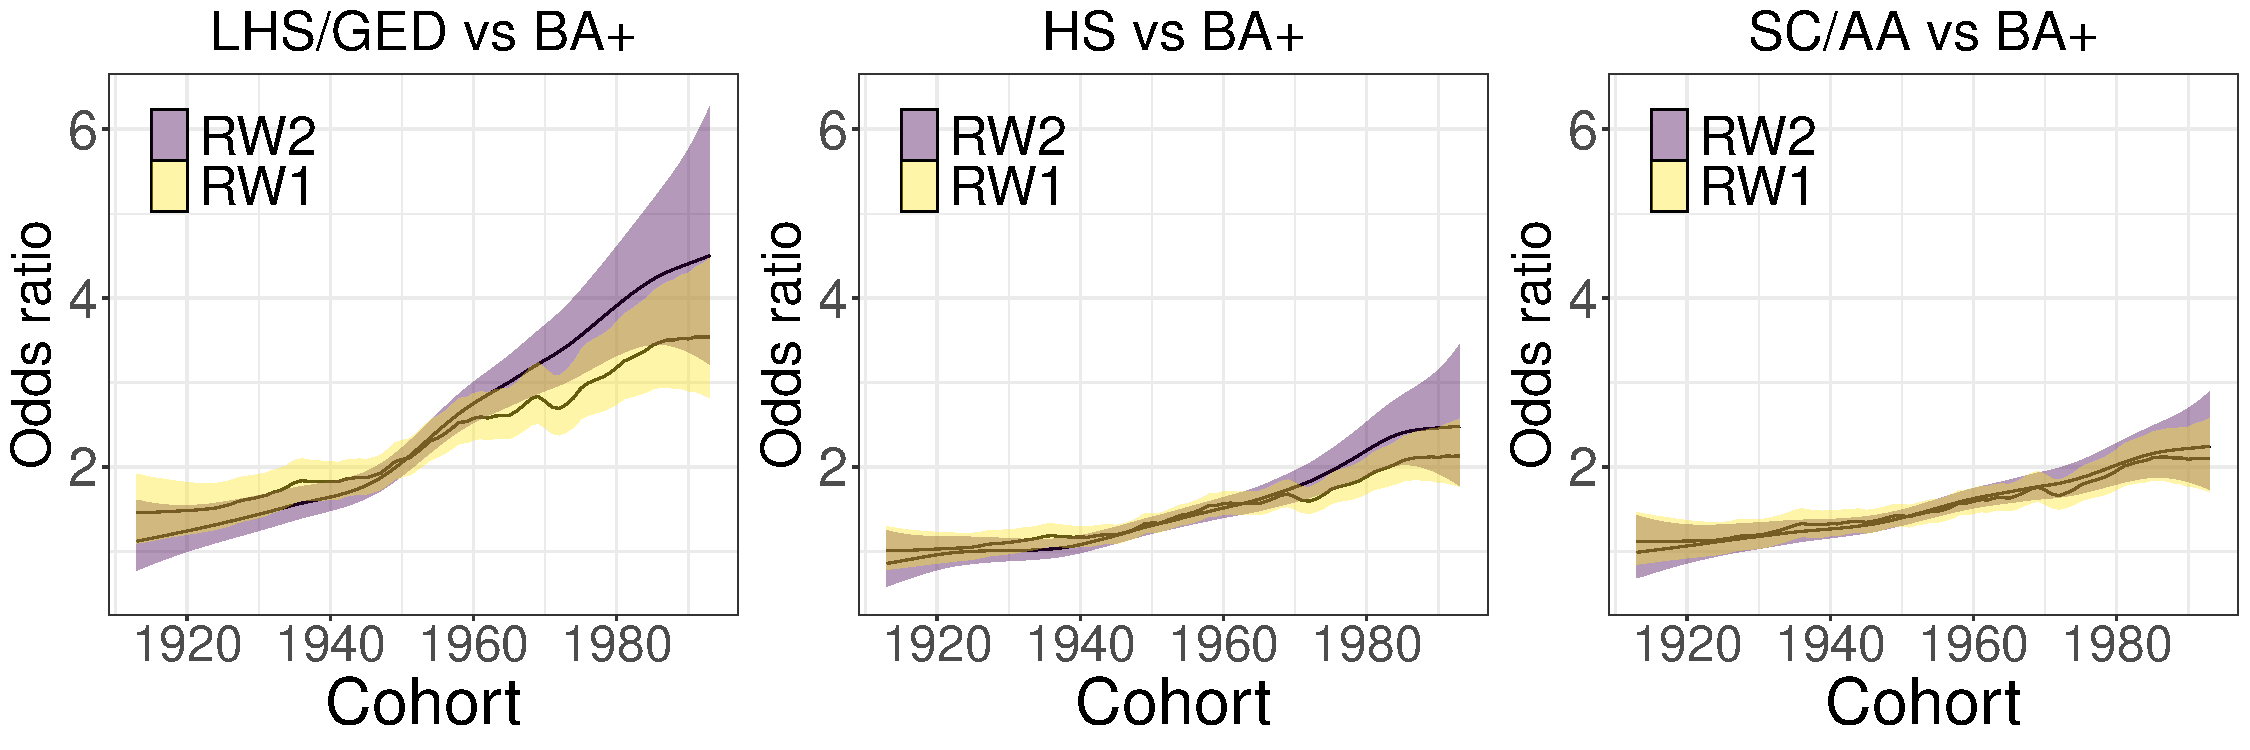
\includegraphics[width=\textwidth]{Figures/lincomb_survey_filtered_cohort_f_rw2.pdf}
    \end{subfigure}
    \caption{The posterior estimated median odds-ratio over \textbf{(a)} age and \textbf{(b)} cohort, for different levels of attained education with respect to the highest level of education along with $95\%$ credible intervals. The trends are shown for two latent field priors (RW1 and RW2) placed on each temporal component in the latent field. A PC$(10,0.01)$ prior is placed on the standard deviation of each component in the RW2 prior, and the EK prior was used in the model with RW1 priors on the latent field. In these aPc models, data from the female, white, U.S-born population was used, and the complex survey design was accounted for. }
    \label{figure:Application1:rw2_f_fil}
\end{figure}

\begin{figure}[h!]
    \centering
    \begin{subfigure}[b]{\textwidth}   
        \centering 
        \caption[]%
        {}    
        \label{figure:Application1:rw2_age_m_fil}
        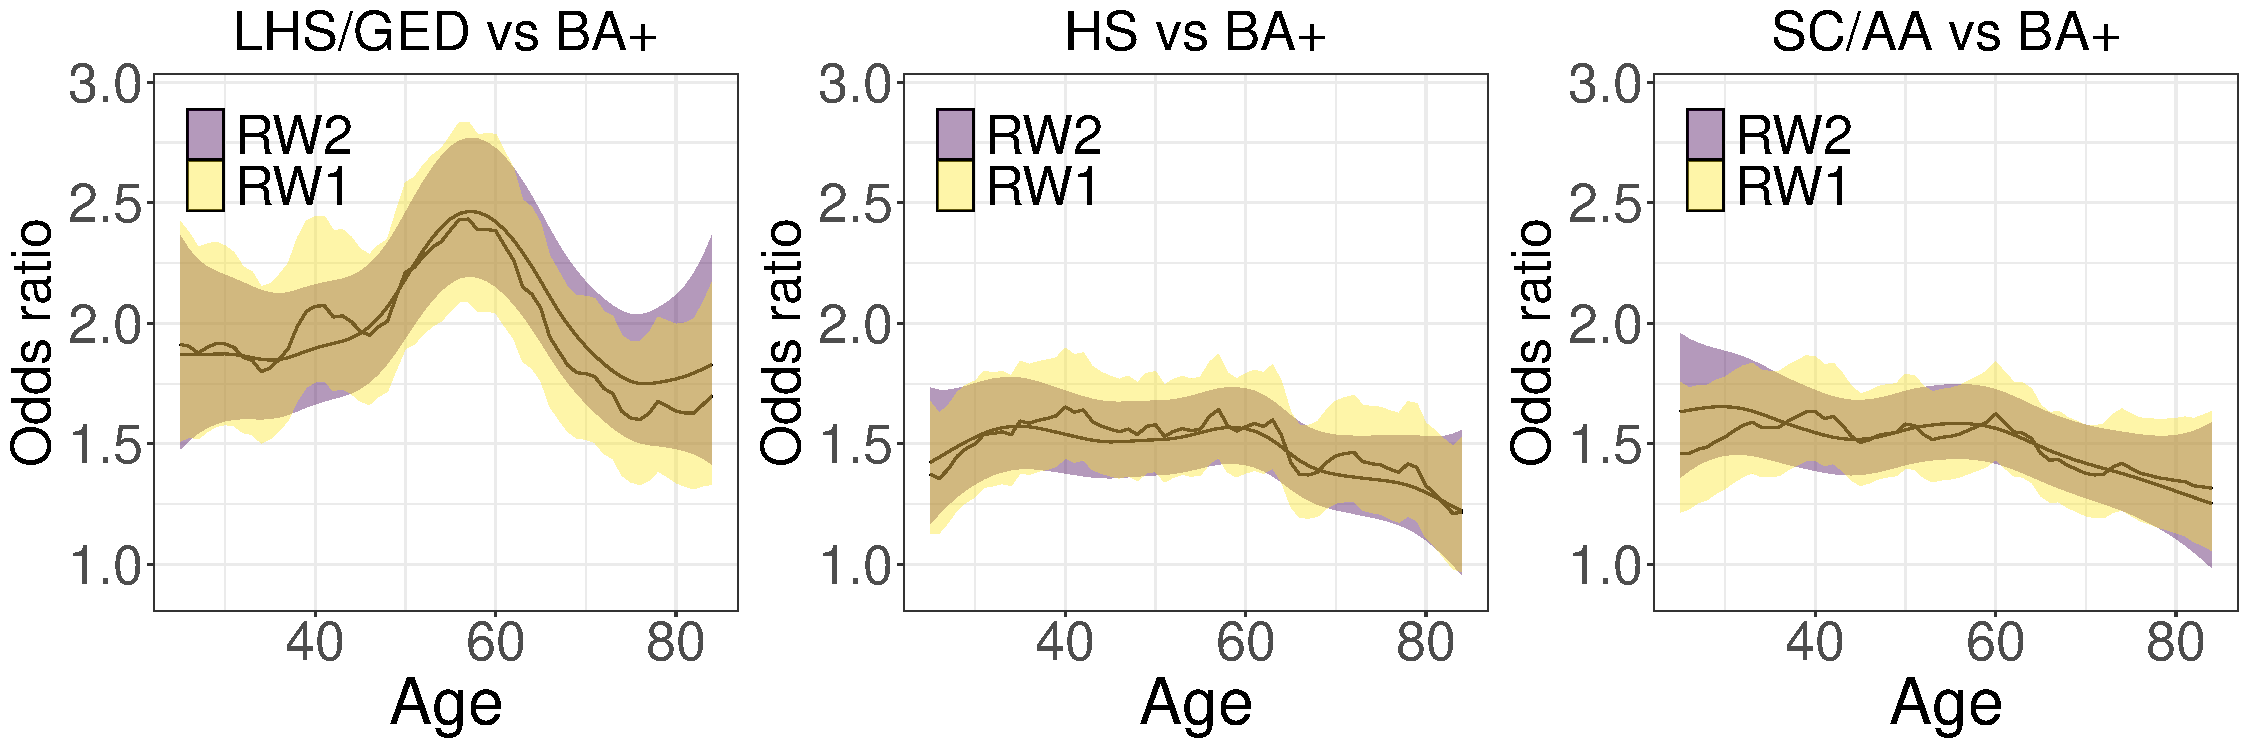
\includegraphics[width=\textwidth]{Figures/lincomb_survey_filtered_age_m_rw2.pdf}
    \end{subfigure}
    \vskip\baselineskip\vspace{-0.3cm}
    \begin{subfigure}[b]{\textwidth}   
        \centering 
        \caption[]%
        {}    
        \label{figure:Application1:rw2_cohort_m_fil}
        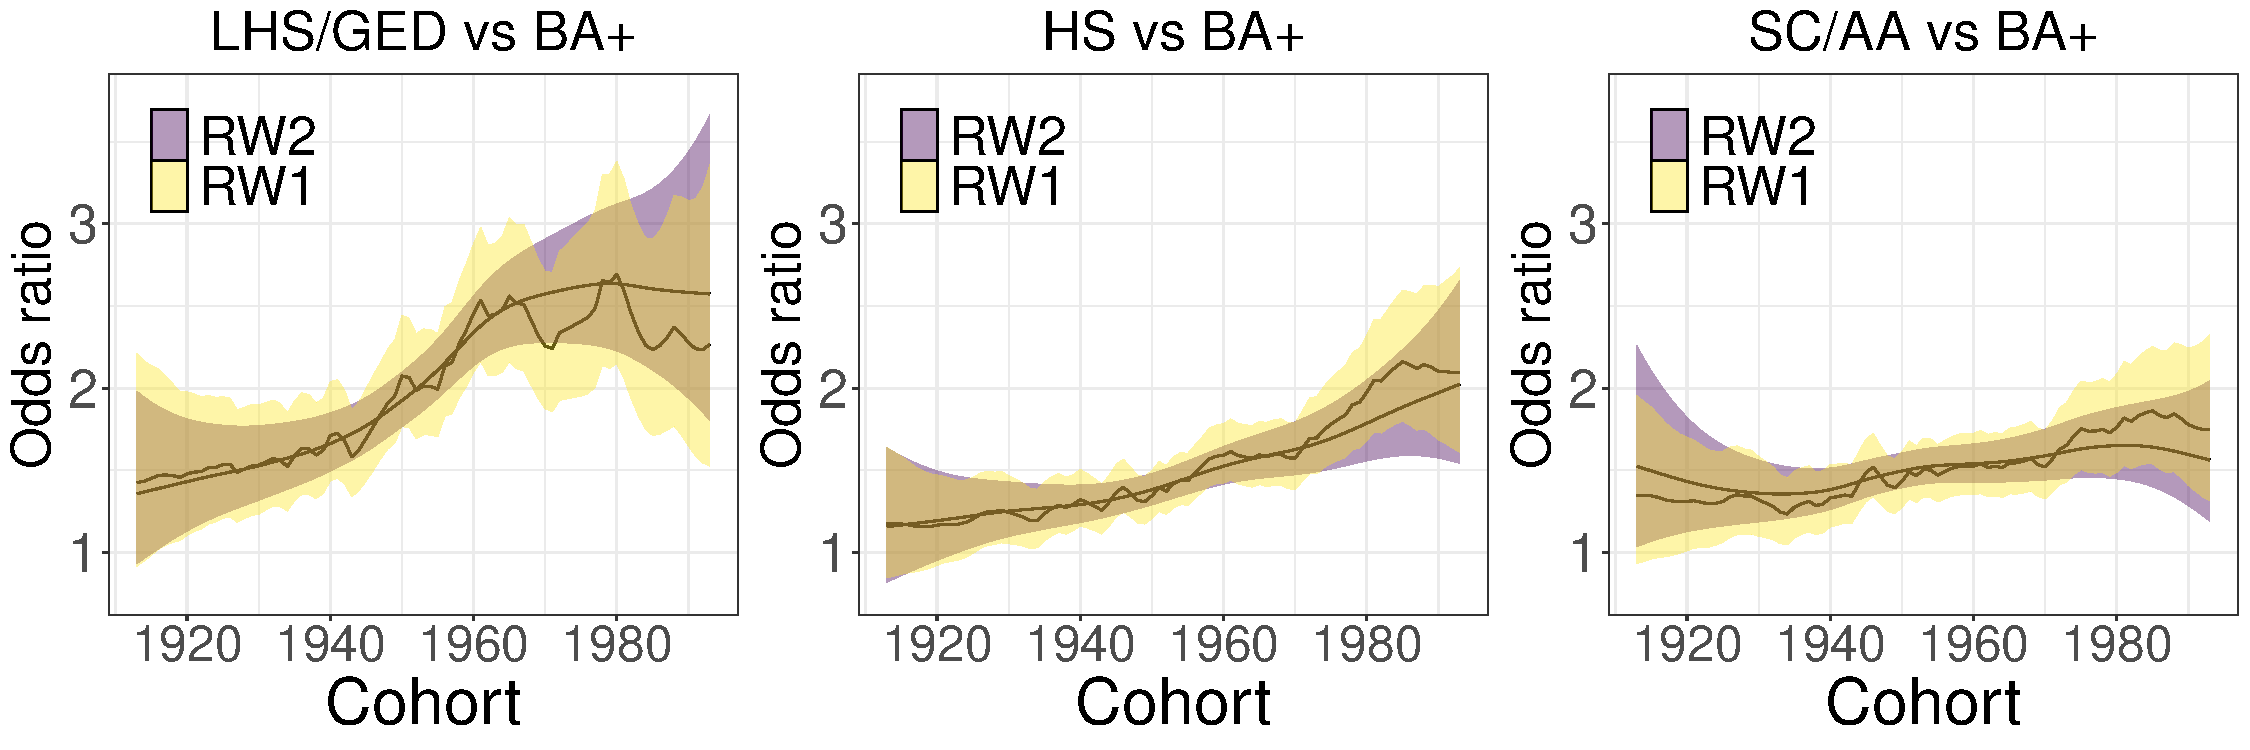
\includegraphics[width=\textwidth]{Figures/lincomb_survey_filtered_cohort_m_rw2.pdf}
    \end{subfigure}
    \caption{The posterior estimated median odds-ratio over \textbf{(a)} age and \textbf{(b)} cohort, for different levels of attained education with respect to the highest level of education along with $95\%$ credible intervals. The trends are shown for two latent field priors (RW1 and RW2) placed on each temporal component in the latent field. A PC$(10,0.01)$ prior is placed on the standard deviation of each component in the RW2 prior, and the EK prior was used in the model with RW1 priors on the latent field. In these aPc models, data from the male, white, U.S-born population was used, and the complex survey design was accounted for. }
    \label{figure:Application1:rw2_m_fil}
\end{figure}

\FloatBarrier
\subsubsection{Details on implementation in \texttt{R}}
\label{appendix:A2:implementaion}
To obtain the estimated probabilities at the logit scale along with estimates of the variance, the \texttt{survey} package in \texttt{R} was used. The package takes the data on an individual specific level and computes estimates of $\pi_{ije}$ and $\sigma^2_{ije}$ for each stratum according to the provided strata using the provided weights. In \texttt{R}, the survey design is specified by
\begin{lstlisting}
des<-svydesign(ids= ~1, strata= ~age+period+education,
                 weights=~sampweight, data = data)
\end{lstlisting}
where the strata denotes the indices $i$, $j$ and $e$ as age, period and education, and the sample weights are provided as \texttt{sampweight} in the data object. The argument \texttt{ids=~1} is required to specify that there are no clusters in the data to correct for. The estimates are then obtained by
\begin{lstlisting}
prevs=svyby(~backpain, 
            by=~education+age+period,
            design=des, FUN=svymean)
\end{lstlisting}
The weighted sample estimators are then transformed by the logit function in Equation \eqref{eqn:logit}, and the variance in Equation \eqref{eqn:asymptoticDistribution} is computed from the weighted sample estimator and the standard deviance estimates. 

To fix the variances, the precision of the latent field was set to $1$ for all observations by supplying \texttt{INLA} with the option \texttt{control.family = list(hyper = list(prec = list(initial = log(1), fixed = T)))}, and then scaled by the transformed precisions using the \texttt{scale} option in the INLA call.

\begin{lstlisting}
    result = inla(formula = your_formula, 
                  data = your_data, 
                  family = "gaussian", 
                  control.family = list(
                    hyper=list(
                      prec=list(
                        initial = log(1), fixed = T))),
                  scale = scale)
\end{lstlisting}






